\documentclass[]{amsart}
\usepackage[]{graphicx}
\usepackage[]{listings}


\begin{document}
\title{title}
\author{author}


\maketitle



\section{examples/tex/blank.tex} 
 \begin{lstlisting}[] 
 \documentclass[]{article}
\usepackage[]{graphicx}
\usepackage[]{hyperref}


\begin{document}
\title{title}
\author{author}

\today
\maketitle




\end{document}
  
 \end{lstlisting} 
  
 \section{examples/tex/with\_image.tex} 
 \begin{lstlisting}[] 
 \documentclass[]{amsart}
\usepackage[]{graphicx}
\usepackage[]{hyperref}


\begin{document}
\title{title}
\author{author}

\today
\maketitle



\includegraphics[]{examples/img/ss.png} 

\end{document}  
 \end{lstlisting} 
  
 \section{examples/tex/source\_code.tex} 
 \begin{lstlisting}[] 
   
 \end{lstlisting} 
  
 \section{examples/tex/options.tex} 
 \begin{lstlisting}[] 
 \documentclass[]{amsart}
\usepackage[]{graphicx}


\graphicspath{{../img}, } 
\begin{document}
\title{title}
\author{author}


\maketitle



\begin{figure}[h] 
 \centering 
 \includegraphics[scale = 0.5, ]{ss.png} 
 
 \caption{this is a caption} 
 \end{figure} \begin{figure}[h] 
 \centering 
 \includegraphics[scale = 0.5, ]{ss.png} 
 
 \caption{this is a caption} 
 \end{figure} \begin{figure}[h] 
 \centering 
 \includegraphics[scale = 0.5, ]{ss.png} 
 
 \caption{this is a caption} 
 \end{figure} 
\end{document}  
 \end{lstlisting} 
  
 \section{examples/collate.rs} 
 \begin{lstlisting}[] 
 use std::error::Error;
use std::fs::File;
use std::io::Write;

use rust_texas::prelude::*;

// walkdir is a dev dependency, and you can implement custom walkdir-ish iterators for your own use case.
use walkdir::WalkDir;

/// We'll put all of texas' example code in a pdf.
///
/// Ideally, you'd be doing this for a bunch of markdown files or text files, but
/// it seemed easier to demonstrate this way. That said, it's still a somewhat complex example.
fn main() -> Result<(), Box<dyn Error>> {
    let mut q = File::create("examples/tex/source_code.tex")?;
    let mut doc = document!("amsart");
    doc.disable_hyperref();

    // Using the listings package, because we're making a source code pdf.
    doc.new_package(Package::new("listings"));

    // The final, NEW, function from the Populate trait is attach_iter. Here, we feed it an iterator over
    // components, namely one section per file in the examples directory. 
    doc.attach_iter(WalkDir::new("examples").into_iter().filter_map(|x| {
        let x = x.ok()?;
        if x.metadata().unwrap().is_dir() {
            None
        } else {
            let fname = x.into_path();
            let fname = fname.to_str().unwrap();

            // This reads the contents of a file and dumps it (raw) into a TextChunk component with TextType::Normal.
            // At this stage, it's just a string.
            let buf = TextChunk::from_file(&fname).ok()?;

            // Because this is source code, we'll put it in an lstlisting environment.
            let mut vb = Environment::new("lstlisting");
            // And embed buf in the lstlisting.
            vb.attach(Component::TextChunk(buf)).ok()?;

            // We'll create a new section for each file, for no particular reason.
            let mut sec = section!(&fname);
            sec.attach(Component::Environment(vb)).ok()?;
            Some(sec)
        }
    }))?;

    writeln!(q, "{}", doc.to_string())?;

    Ok(())
}
  
 \end{lstlisting} 
  
 \section{examples/options.rs} 
 \begin{lstlisting}[] 
 use std::error::Error;
use std::fs::File;
use std::io::Write;

use rust_texas::prelude::*;

/// This example embeds the screenshot of this file in the pdf.
fn main() -> Result<(), Box<dyn Error>> {
    let mut q = File::create("examples/tex/options.tex")?;
    let mut doc = document!("amsart");
    doc.disable_hyperref();

    // Add a directory in the graphics path for graphicx
    doc.push_gpath("../img");

    // Create a new Image. The macro image! gives us a Component, but we want the inner struct.
    let mut img = Image::new("ss.png");

    // Add the option!
    img.add_option("scale = 0.5");

    // Include the image in a figure enviroment.
    let mut ss = Figure::from_img(img, "this is a caption".to_string());
    ss.add_option("h");

    // attach_vec, again from the Populate trait, makes attaching multiple objects much more convenient.
    doc.attach_vec(vec![Component::Figure(ss); 3])?;

    write!(q, "{}", doc.to_string())?;

    Ok(())
}
  
 \end{lstlisting} 
  
 \section{examples/blank\_document.rs} 
 \begin{lstlisting}[] 
 use std::error::Error;
use std::fs::File;
use std::io::Write;

use rust_texas::prelude::*;

fn main() -> Result<(), Box<dyn Error>> {
    let mut q = File::create("examples/tex/blank.tex")?;
    let mut doc = Document::new(DocumentClass::new("article"));
    doc.set_md("title", &["author"]);
    // Uncomment to not include the hyperref and graphicx packages, which are included by default.
    // doc.disable_graphicx();
    // doc.disable_hyperref();
    writeln!(q, "{}", doc.to_string())?;
    Ok(())
}
  
 \end{lstlisting} 
  
 \section{examples/image.rs} 
 \begin{lstlisting}[] 
 use std::error::Error;
use std::fs::File;
use std::io::Write;

use rust_texas::prelude::*;

/// This example embeds the screenshot of this file in the pdf.
fn main() -> Result<(), Box<dyn Error>> {
    let mut q = File::create("examples/tex/with_image.tex")?;
    // We can use the document! macro to create a document, resulting in more concise code.
    // texas supports multiple document classes
    let mut doc = document!("amsart");

    // We can add things to a document using the attach method from the Populate trait.
    doc.attach(image!("examples/img/ss.png"))?;

    write!(q, "{}", doc.to_string())?;

    Ok(())
}
  
 \end{lstlisting} 
  
 
\end{document}
